\section{Overview of Plasma Physics}
A \emph{plasma} is a quasi-neutral gas of ions, electrons, and neutral particles, which exhibit collective behavior. Plasmas can behave in similar ways to a conventional fluid -- they can flow, they can be compressible, they can be turbulent, and so on -- however the addition of charged particles facilitates many behaviors unique to a plasma. Charged particles can interact with each other not just through ballistic collisions, but at a distance through electromagnetic forces. The bulk motion of a plasma can be manipulated through electric and magnetic fields; conversely a plasma can have a substantial effect on the propagation of radio waves passing through it. 

A plasma can be analyzed in several different domains: Single particle motion; fluid approximations; and full kinematic solutions. In this work we treat the motions of electrons in the single particle domain, which is a natural choice for the sparse densities and small gyroradii of radiation belt electrons. To understand the behavior of radio waves propagating through a plasma, we treat the background as a smooth dielectric medium. 

\subsection{Single Particle Motion}
\label{section:single_particle_motion}
The high energies and sparse densities of the radiation belts lend themselves very well to a single-particle approximation. Many of the basic behaviors and quantities in plasma physics can be understood through studying the motion of a single particle.

The fundamental equation of motion for a charged particle in an electromagnetic field is given by the Lorentz force:
\begin{equation}
\vec{F} = \frac{d\vec{p}}{d\emph{t}} = q(\vec{E} + \vec{v}\times\vec{B})
\label{eqn:lorentz_force}
\end{equation}
Where $q$ represents the particle's charge, $\vec{E}$ and $\vec{B}$ represent the electric and magnetic fields, and $\vec{v}$ the particle's velocity, shown here in a non-relativistic frame.

Electric fields simply apply a force in the direction of the field. However, note that a cross product is perpendicular to both terms -- therefore any forces induced by the magnetic field will be perpendicular to the particle's velocity. The magnetic field is a \emph{conservative} force, in that a stationary magnetic field cannot directly impart energy into a particle, but can alter a particle's trajectory. The particle will therefore have a net drift in the direction of the electric field, while exhibiting a helical motion around the magnetic field.

We can then split the velocity vector into two quantities -- $v_\parallel$ parallel to the magnetic field, and $v_\perp$ perpendicular to the magnetic field.

Two characteristic values arise from this motion: the radius of the particle's rotation around the magnetic field, known as the \emph{gyroradius} or the \emph{Larmor radius}:
\begin{equation}
r_l = \frac{m v_\perp}{qB}
\end{equation}

And the rotation frequency, known as the \emph{gyrofrequency} or \emph{cyclotron frequency}:
\begin{equation}
\omega_c = \frac{v_\perp}{r_l} = \frac{q B}{m} \unit{rad/sec}
\end{equation}

By integrating the particle's momentum over a single gyrorotation, we arrive at a third fundamental quantity known as the magnetic moment, or the \emph{first adiabatic invariant}:
\begin{equation}
\mu = \frac{m v_\perp^2}{2B}
\label{eqn:first_adiabatic_invariant}
\end{equation}

In situations where the magnetic field varies slowly (e.g., on spatial scales much greater than the gyroradius), then $\mu$ remains a constant of motion.

A final parameter to describe a particle's motion is it's \emph{pitch angle}, the angle between the velocities perpendicular and parallel to the magnetic field:
\begin{equation}
\alpha = \mathrm{tan}^{-1}\bigg(\frac{v_\perp}{v_\parallel}\bigg)
\end{equation}

The first adiabatic invariant describes an implicit relationship between the magnetic field strength and a particle's pitch angle at a given point. 
Combining the first adiabatic invariant with conservation of kinetic energy, we can deduce an expression for magnetic trapping -- that is, the magnetic field strength in which a particle exhibiting helical motion along a magnetic field line will turn around at. 
\begin{eqnarray}
& E &= \frac{1}{2}mv^2 \\
& &= \frac{1}{2}m(v_\parallel^2 + v_\perp^2) \\
 & &= \frac{1}{2}mv^2(\mathrm{cos}^2\alpha + \mathrm{sin}^2\alpha)
\end{eqnarray}

At a reflection point, the particle's kinetic energy will be entirely in the perpendicular mode:
\begin{eqnarray}
\frac{v_{\perp0}^2}{B_0} = \frac{v_{\perp1}^2}{B_1} \\
\frac{v^2\mathrm{sin}^2(\alpha)}{B_0} = \frac{v^2}{B_1} \\
\mathrm{sin}^2(\alpha)=\frac{B_0}{B_1} 
\end{eqnarray}

Therefore, a charged particle in a magnetic field will be constrained to rotate around a field line, and bounce back and forth, reflecting where the magnetic field strength increases. A key takeaway is that the reflection point is independent of energy, and depends only on the ratio of magnetic field strengths and the particle's initial pitch angle. An example of this behavior is shown in figure \ref{fig:bottle}.
\begin{figure}[ht]
\begin{center}
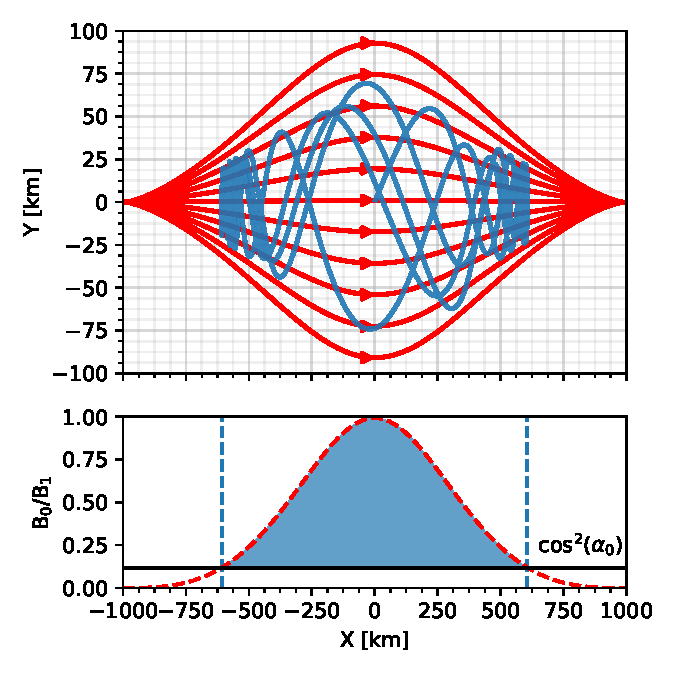
\includegraphics{figures/bottle.pdf}
\caption[An example of a ``magnetic bottle'' particle trap]{An example of a ``magnetic bottle" particle trap. The top plot shows the trajectory of an electron with an initial pitch angle $\alpha_0=20^\circ$. The bottom plot shows the magnetic field ratio $B_0/B_1$, with the particle's reflection points shown as vertical lines. }
\label{fig:bottle}
\end{center}
\end{figure}

\subsection{The Loss Cone}

A magnetic bottle trap need not be linearly-arranged, as it is in figure \ref{fig:bottle}; we require only that the magnetic field be slowly-varying with respect to the particle's gyroradius. The Earth's dipole magnetic field forms a natural and effective particle trap, which dominates the morphology of charged particle populations surrounding the Earth.

The motion of a charged particle in the Earth's magnetic field can be broken into three components: 
\begin{itemize}
\item A rapid gyrorotation around the background magnetic field
\item A ``bouncing'' motion between the north and south poles, with periods ranging from milliseconds to several seconds
\item A slower, longitudinal drift, causing the particles to precess around the earth on the order of minutes to days, resulting from the magnetic field gradient
\end{itemize}

\begin{figure}[ht]
\begin{center}
\includegraphics[draft]{figures/basic_motions.pdf}
% THIS IS THE STANDARD CARTOON OF THE BOUNCE AND DRIFTS...
\caption[Adiabatic motion in the Earth's magnetic field]{Illustration of the various motions exhibited by a charged particle in the Earth's magnetic field}
\label{fig:adiabatic_motions}
\end{center}
\end{figure}

We can average the particle's motion over a single gyrorotation to define a \emph{guiding center}, the trajectory of which follows the background magnetic field line. 

As described previously, a trapped particle's reflection points are defined by the particle's initial pitch angle, and the strength of the magnetic field. In the case of the Earth, however, these turning points are limited in feasibility as well -- for instance, a particle naturally cannot have a reflection point lower than the Earth's surface. Moreover, the Earth's neutral atmosphere becomes exponentially more-dense with decreasing altitude; particles reflecting at an altitude below $\approx 100$ km will encounter a significant neutral molecule population, and stand a very good chance of colliding. A collision with atmospheric constituents can result in the particle losing some, or all, of it's kinetic energy through ionization, and may be completely lost from the system, or return onto a different fieldline \citep{Cotts2011}.

With an understanding of the dense neutral atmosphere, we can define a critical altitude -- 100 km here and in related work -- and thus a critical pitch angle, known as the \emph{loss-cone angle}:
\begin{equation}
\sin \alpha_{lc} = \sqrt{\frac{B(\vec{r})}{B_{h_m}}}
\end{equation}
where $h_m$ is the reflection height, and $B(\vec{r})$ is measured at the reference point -- either the particle's current location for a \emph{local loss cone}, or at the equator along the field line for the \emph{equatorial loss cone}.

\begin{figure}[h]
\begin{center}
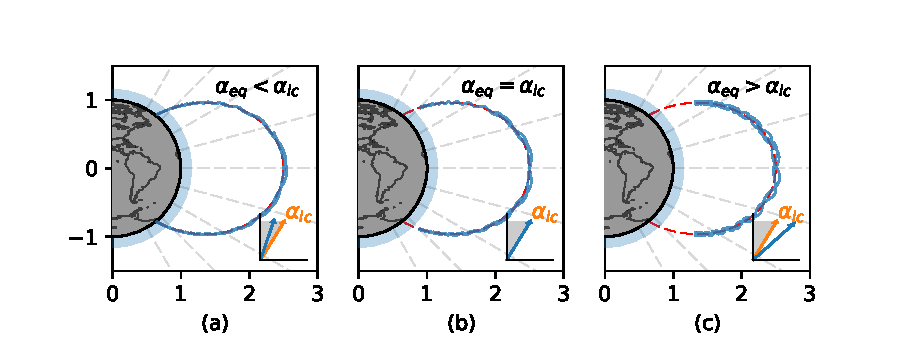
\includegraphics[width=\textwidth]{figures/pitchangle_trapping_3up.pdf}
\caption[Loss cone illustration]{An illustration of the loss cone. The trajectory of a test electron is shown in blue, for three different equatorial pitch angles: (a) a precipitating particle with a pitch angle within the loss cone,  (b) at the edge of the loss cone, and (c), a stably-trapped particle with a pitch angle well outside the loss cone.}
\label{fig:loss_cone_examples}
\end{center}
\end{figure}


In the case of a dipole magnetic field model, we can determine the equatorial loss cone explicitly:
\begin{equation}
\sin \alpha_{lc} = \sqrt{\frac{\zeta_m^3}{\sqrt{1 + 3 (1 - \zeta_m)}}} \qquad \zeta_m = (R_e + h_m) / (L R_e)
\end{equation}
where $R_e = 6371$ km is the radius of the Earth, and L is the \emph{L-shell} of interest (see section \ref{section:dipole_model}).



\paragraph{Bounce and Drift Loss Cones}
We have discussed what is known as the \emph{bounce loss cone}. In literature, there is often mention of both the bounce loss cone and a \emph{drift loss cone}. The drift loss cone is the largest loss cone along the same L-shell, as it varies longitudinally -- conceptually, as a particle drifts longitudinally, it may encounter a different loss cone, and could precipitate at certain longitudes, but not others. 

Under a simple dipole magnetic field model, the two are identical. Within this dissertation, we primarily work with a dipole magnetic field model, and consider only the bounce loss cone.

\subsection{Waves in Plasmas}
Previously, we have described the motion of a charged particle under the influence of an electromagnetic field. the single-particle approximation provides enormous insight into the dynamics of a sparsely-populated plasma. Next, we must consider the inverse system -- how the charged particles in a plasma dictate the characteristic behaviors of an electromagnetic wave propagating through it.

An electromagnetic wave can accelerate a charged particle; conversely, an accelerating or decelerating particle induces its own electromagnetic field. It would seem, then, that the behavior of an electromagnetic field in a plasma is simply the summation of the contributions of each particle and some incident wave source. However, the complexity of this brute-force approach quickly becomes intractable for even a handful of particles. The universal approach taken then is to abstract the complicated interplay of waves and particles into a wave moving through a dielectric medium, described only by the various constituent densities, temperatures, and background field intensities within a given volume. 

As with any electromagnetic problem, we begin with Maxwell's equations -- shown here in their non-relativistic, differential form, in SI units:

\begin{eqnarray}
&\nabla \cdot \vec{E}& = \frac{\rho}{\epsilon_0} \label{eqn:maxwell1}\\
&\nabla \cdot \vec{B}& = 0 \label{eqn:maxwell2}\\
&\nabla \times \vec{E}& = -\frac{\partial \vec{B}}{\partial t} \label{eqn:maxwell3}\\
&\nabla \times \vec{B}& = \mu_0 \vec{J} + \frac{1}{c^2}\frac{\partial \vec{E}}{\partial t} \label{eqn:maxwell4}
\end{eqnarray}

$\vec{E}$ and $\vec{B}$ denote the electric and magnetic fields; $\mu_0$ and $\epsilon_0$ denote the magnetic permeability and electric permittivity of free space; and $c=\sqrt{\frac{1}{\mu_0\epsilon_0}}$ is the speed of light. The terms $\rho$ and $\vec{J}$ represent the local charge density and current density, both of which may be functions of position and time.

By taking the curl of equation \ref{eqn:maxwell3} and substituting in the time derivative of equation \ref{eqn:maxwell4}, and making use of the vector identity $\nabla \times \nabla \times \vec{E} = \nabla(\nabla \cdot \vec{E}) - \nabla^2\vec{E}$, we have:

\begin{equation}
\nabla^2\vec{E} - \frac{\nabla\rho}{\epsilon_0} = \mu_0 \frac{\partial \vec{J}}{\partial t} + \frac{1}{c^2}\frac{\partial^2\vec{E}}{\partial t^2}
\label{eqn:dielectric_tensor_derivation_1}
\end{equation}

In the absence of charges or currents ($\rho=0$, $\partial\vec{J}/\partial t=0$), the equation reduces to the free-space wave equation:
\begin{equation}
\nabla^2\vec{E} = \frac{1}{c^2}\frac{\partial^2\vec{E}}{\partial t^2}
\end{equation}

Next, we linearize the system and search for harmonic perturbations of the form:
\begin{eqnarray}
\vec{E(\vec{r},t)} = \vec{E_1}e^{{i (\omega t - \vec{k}\cdot \vec{r}})} \label{eqn:linear1}\\ 
\vec{B(\vec{r},t)} = \vec{B_0} + \vec{B_1}e^{{i (\omega t - \vec{k}\cdot \vec{r}})} \label{eqn:linear2}\\
\vec{J(\vec{r},t)} = \vec{J_1}e^{{i (\omega t - \vec{k}\cdot \vec{r}})}\label{eqn:linear3} 
\end{eqnarray}

where $\omega$ is the wave angular frequency, $\vec{k}$ is the wave vector, or spatial frequency, and $\vec{r}$ is the spatial coordinate. Two fundamental parameters of an electromagnetic wave are the \emph{phase velocity}, $\omega/k$, and the \emph{group velocity}, $\partial\omega/\partial k$. The relation between the temporal and spatial frequencies is known as the \emph{dispersion relation}.

From here we follow the derivation and convention used by \cite{Stix1992} and \cite{Bittencourt2004}. In general, a plasma is comprised of several different species of constituent particles -- positively and negatively charged particles necessary to maintain a quasi-neutral plasma. While the dispersion relations of different species cannot be simply added, their effects can be summed to form the displacement current $\vec{J}$:
\begin{equation}
\vec{J} = \sum_s\vec{J_s} = \sum_s n_s q_s \vec{u_s}
\label{eqn:J}
\end{equation}
where $n$, $q$, and $\vec{u}$ represent the (number) density, charge, and velocity of a particular species $s$. 

We make the assumption that the plasma is \emph{cold} -- that is, that the velocities of each species $\vec{u_s}$ have a single value each. Were we to relax this assumption, each species density would have a distribution function in both position and momentum, $n=n(\vec{r},\vec{p})$; the total current would then be an integration over momentum for each species. For a treatment of a hot plasma, see the work by \cite{Sazhin1993}.

Next, we note that, in a cold plasma assumption, the Lorentz force (equation \ref{eqn:lorentz_force}) can be written for each species:
\begin{equation}
m_s\frac{d\vec{u_s}}{dt} = q_s\big(\vec{E} + \vec{u_s}\times\vec{B}\big) 
\label{eqn:lorentz_2}
\end{equation}
Combining equations \ref{eqn:linear1} -- \ref{eqn:linear3}, \ref{eqn:J}, and \ref{eqn:lorentz_2}, and assuming a coordinate system with the background magnetic field $\vec{B_0}$ aligned with the z-axis, we arrive at an expression for the \emph{cold-plasma dielectric tensor}:

\begin{equation}
\mvec{\epsilon}\cdot\vec{E}=\begin{pmatrix}
S & -iD & 0 \\
iD & S & 0 \\
0 & 0 & P \end{pmatrix}\begin{pmatrix}E_x \\ E_y \\ E_z\end{pmatrix}
\end{equation}

The various summations over each constituent species are incorporated into the so-called Stix parameters (\cite{Stix1992}):
\begin{eqnarray}
S =\frac{1}{2}(R + L) \qquad D = \frac{1}{2}(R - L)
\label{eqn:stix_params_1}
\end{eqnarray}
\begin{equation}
R = 1 - \sum_s\frac{\omega_{ps}^2}{\omega(\omega + \omega_{cs})}; \quad L = 1 - \sum_s\frac{\omega_{ps}^2}{\omega(\omega - \omega_{cs})}; \quad P = 1 - \sum_s\frac{\omega_{ps}^2}{\omega^2}
\label{eqn:stix_params_2}
\end{equation}

where $\omega_{ps} = n_sq_s^2/{\epsilon_0 m_s}$ and $\omega_{cs}=q_sB_0/m_s$ are the plasma and cyclotron frequencies for species $s$.

\subsubsection{Dispersion Relation}
With the dielectric tensor now determined, we can derive the relationship between $\omega$ and $\vec{k}$, known as the dispersion relation. Equation \ref{eqn:dielectric_tensor_derivation_1} can be written as:
\begin{equation}
\mvec{\eta}\times \mvec{\eta} \times \vec{E} +  \mvec{\epsilon}\cdot\vec{E} = 0
\end{equation}
where $\mvec{\eta} = \vec{k}c/\omega$ is the wave refractive index. Assuming a wave propagating with some angle $\theta$ between $\mvec{\eta}$ and the background magnetic field, we arrive at:
\begin{equation}
\begin{pmatrix}
S - \eta^2\cos^2\theta & -iD & \eta^2\cos{\theta}\sin{\theta} \\
iD & S - \eta^2 & 0 \\
\eta^2\cos{\theta}\sin{\theta} & 0 & P - \eta^2\sin^2{\theta} \end{pmatrix}\begin{pmatrix}E_x \\ E_y \\ E_z\end{pmatrix} = 0
\label{eqn:dispersion_relation_matrix}
\end{equation}

Taking the determinant of \ref{eqn:dispersion_relation_matrix} yields the \emph{cold-plasma dispersion relation}:

\begin{eqnarray}
&A\eta^4 - B\eta^2 + C &= 0 \label{eqn:disp_rln}  \\
&A& = S \sin^2\theta + P\cos^2\theta \\
&B& = RL\sin^2\theta + PS(1 + \cos^2\theta) \\
&C& = PRL
\end{eqnarray}

Equation \ref{eqn:disp_rln} is biquadratic -- we can solve for $\eta^2 = k^2c^2/\omega^2$ using the quadratic formula.

Finally, it is worth noting that when considering a single-species plasma (e.g., electrons only), equation \ref{eqn:disp_rln} reduces to the well-known \emph{Appleton-Hartree Equation} (\cite{Appleton1932}):


\begin{equation}
\eta^2 = 1 - \frac{\frac{\omega_{pe}^2}{\omega^2}}{1 - \frac{\omega_{ce}^2\sin^2\theta}{2(\omega^2 - \omega_{pe}^2)} \pm\big[\big(\frac{\omega_{ce}^2\sin^2\theta}{2(\omega^2 - \omega_{pe}^2)}\big)^2 + \frac{\omega_{ce}^2}{\omega^2}\cos^2\theta\big]^{1/2}}
\end{equation}

%For a simpler derivation of the Appleton-Hartree equation alone, see the classic, approachable text by \cite{Chen1983}.  %% (CHEN DOESN'T SEEM TO DO IT x.x) 

The dispersion relation in equation \ref{eqn:disp_rln} reveals a wealth of information about the characteristics of waves in plasmas. For various plasma densities and background magnetic field strength, we can infer which wave frequencies may propagate, if any, and which wave polarizations. Through the remainder of this work, we will be concerned with the \emph{Whistler} mode -- a right-hand, circularly-polarized (RHCP) wave. Within a typical magnetospheric plasma, the Whistler mode spans the VLF band, roughly between 30 Hz and 300 kHz.

Figure \ref{fig:whistler_mode_dispersion} shows a typical dispersion relation for a magnetospheric plasma (L $\approx$ 2) by plotting frequency vs wavenumber ($\eta = k c/\omega$). The Whistler mode is the lower branch of the RHCP mode.
\begin{figure}[!ht]
\begin{center}
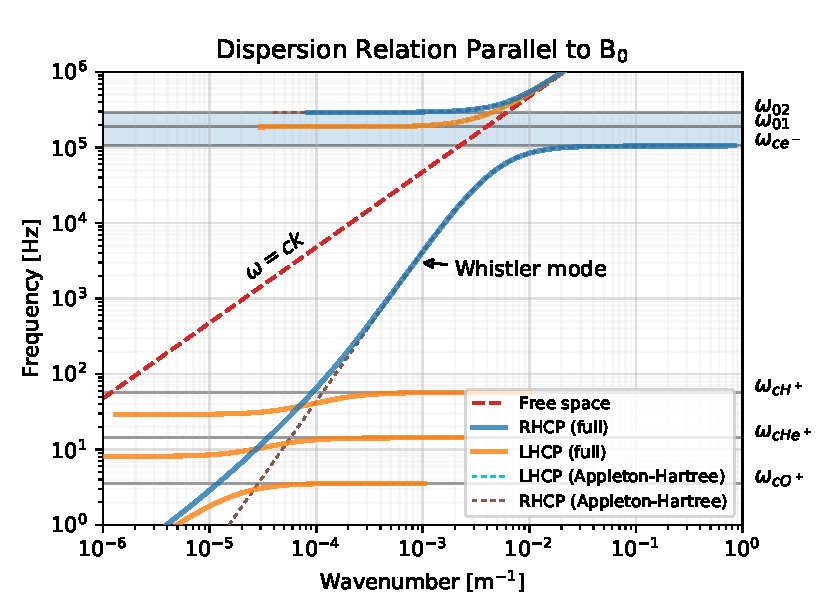
\includegraphics{figures/omega-k_diagram_parallel}
\caption[An $\omega$-K diagram for the cold, four-component dispersion relation, for parallel propagation at L$\approx$3]{An $\omega$-K diagram for the cold plasma dispersion relation, shown here for a wave propagating parallel to $\vec{B}$, in four-component plasma with $N_e \approx  6\E{8}\,e^-/m^3$, and $B\approx 4\,\mu T$. For higher frequencies the dispersion relation asymptotes to the free-space solution, with slope $c$. The Whistler mode is the right-hand, circularly-polarized mode which spans the majority of the frequency band. The shaded region marks the characteristic band in which the right-hand mode cannot propagate. At lower frequencies, the left-hand circular mode resonates with the various ion constituents,  known as the \emph{Ion Cyclotron} modes.}
\label{fig:whistler_mode_dispersion}
\end{center}
\end{figure}